Let
\begin{align}
\vec{A} = \myvec{1 \\ 2 \\ 3} , 
\vec{B} = \myvec{-1 \\ 0 \\0} , 
\vec{C} = \myvec{0 \\ 1 \\ 2}.
\end{align}
Then, 
\begin{align}
\vec{A} - \vec{B} = \myvec{2 \\ 2 \\  3} 
\\
\vec{C} - \vec{B} = \myvec{1 \\ 1 \\ 2}
\end{align}
Thus, 
\begin{align}
\vec{B} &= \cos^{-1}\myvec{{\frac{(\vec{A-B})^T\vec{(C-B)}}{\norm{\vec{A-B}}\norm{\vec{C-B}}}}}
&= \cos^{-1}\myvec{\frac{10}{\sqrt{17}\sqrt{6}}}
\\
& = 66.15
\end{align}
See Fig. \ref{vectors/2/5/fig: triangle ABC}
\begin{figure}[!ht]
\centering
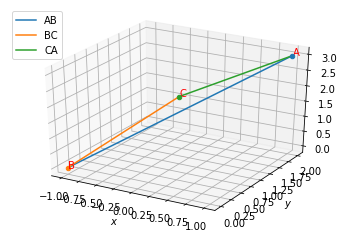
\includegraphics[width=\columnwidth]{solutions/su2021/2/5/download (4).png}
\caption{$\triangle$ABC}
\label{vectors/2/5/fig: triangle ABC}	
\end{figure}
